\documentclass[pdftex, 11pt]{article}

\usepackage[pdftex]{graphicx}
\usepackage{listings}
\usepackage{fancyhdr}
\usepackage{lastpage}
\usepackage{fullpage}
\usepackage{color}
\usepackage[pdftex,bookmarks=true,colorlinks=true,linkcolor=blue]{hyperref}

%this sets the line at the header
\setlength{\headheight}{15.2pt}

\newcommand{\HRule}{\rule{\linewidth}{0.5mm}}

% This is all for formatting and making the Table of Contents according to 
% spec. Don't play with it.
\makeatletter
\renewcommand\l@section[2]{%
  \ifnum \c@tocdepth >\z@
    \addpenalty\@secpenalty
    \addvspace{1.0em \@plus\p@}%
    \setlength\@tempdima{1.5em}%
    \begingroup
      \parindent \z@ \rightskip \@pnumwidth
      \parfillskip -\@pnumwidth
      \leavevmode \bfseries
      \advance\leftskip\@tempdima
      \hskip -\leftskip
      #1\nobreak\ 
      \leaders\hbox{$\m@th\mkern \@dotsep mu\hbox{.}\mkern \@dotsep mu$}
     \hfil \nobreak\hb@xt@\@pnumwidth{\hss #2}\par
    \endgroup
  \fi}
\makeatother



\begin{document}

%import the title page
\begin{titlepage}
	\begin{center}

		% Upper part of the page
		\textsc{\LARGE University of Nevada, Reno}\\[.5cm]
		
\includegraphics[width=0.15\textwidth]{./logo.png}\\[.5cm]

		\textsc{\large CS 302 | Data Structures } \\[.5cm]

		% Title
		\HRule \\[0.4cm]
		{ \huge \bfseries Assignment \#3}\\[0.4cm]

		\HRule \\[1.5cm]

		% Author and supervisor
		\begin{minipage}{0.4\textwidth}
			\begin{flushleft} \large
				\emph{Students:}\\
				Joshua \textsc{Gleason}\\
				Josiah \textsc{Humphrey}
			\end{flushleft}
		\end{minipage}
		\begin{minipage}{0.4\textwidth}
			\begin{flushright} \large
				\emph{Instructor:} \\
				Dr. George \textsc{Bebis}
			\end{flushright}
		\end{minipage}

		\vfill

		% Bottom of the page
		{\large \today}

	\end{center}

\end{titlepage}


%headers, footers, and table of contents
\pagestyle{fancy}
\renewcommand{\sectionmark}[1]{\markright{\thesection}}
\rhead{Page \thepage\ of \pageref{LastPage}}
\lhead{}
\lfoot{CS 302 | Spring 2010}
\cfoot{}
\renewcommand{\footrulewidth}{0.4pt}

\tableofcontents

\listoffigures
\newpage

\lhead{Joshua Gleason \& Josiah Humphrey}
\rhead{Page \thepage\ of \pageref{LastPage}}
\rfoot{Section\ \rightmark}
\cfoot{}
\lfoot{CS 302 | Spring 2010}
\renewcommand{\footrulewidth}{0.4pt}

\section{Introduction}

In this assignment, the students were asked to make an image class that manipulated a Portable Gray Map (PGM) image
in various ways. This was to be accomplished using dynamic 2D arrays and other tools that were learned in previous CS courses.

One of the first problems faced was how to use the supplied read and write image files.
These functions were provided to simplify the build process as they allowed the students to concentrate 
on the manipulation of the images.

After reading and writing images was mastered, the students undertook the bulk of the assignment which was to
manipulate the images that had been read in with the supplied read function. This required the knowledge of
manipulating dynamic 2D arrays. Dynamic 2D arrays was a new tool for the students' C++ repertoire, but the
students soon came to understand the benefits of dynamic 2D arrays.

The assignment also required the use of constructors, destructors, copy constructors, and operator overloading,
These topics were review from CS 202, but the use of them refreshed the students minds on how they work
and to their purposes.

The students also extensively documented their program and made it as easy as possible to understand what
was happening in the various algorithms that were implemented. The students realize that commenting
and documenting the source code for projects is extremely important and is essential to the success of
a powerful programmer.

\section{Use of Code}

The use of the program should be very intuitive. The user must use the arrow keys to scroll in the menu and press enter
to select some option. The menu will then pop up windows and message boxes depending on the user's selection and the
user's input. This provides for a very effective setup and takes the burden out of trying to look at the keyboard and
the menu for key choices in a simple menu. Our menu uses ncurses to accomplish the scrolling menu. The students adapted
a ncurses API written by Micheal Leverington from CS 135 to implement a simple curses menu at the beginning, but after
all of the functions were completed, the students decided to make a more robust menu capable of scrolling. This was not
required, but was done for aesthetic reasons and for the experience that it allowed the students.

The image class that was implemented has all of the requirements for the functions. Each function is defined exactly
like Dr. Bebis wanted them to be defined and the coders adapted their coding style to match what Dr. Bebis expected. The
code is built fairly modular and most of the time expects the class user to bounds and error check before information is
sent to the class. There is some rudimentary error checking in the class itself, but it only prevents the most foul and
gross errors. The class is also setup to throw string objects in the case of an error. These thrown strings must be
caught in the driver, so it is up to the class user to implement the catches for these thrown strings. Strings were used
as the errors because of their ease of use and ease of manipulating them by the class user. 

The file IO functions that were provided by Dr. Bebis have been combined into a single file pair (.cpp and .h) called
imageIO. This allows a much more unified and modular approach to the use of the image IO features. It also makes
including the functions much easier to include into multiple source files.

Whenever a new image is needed by the user of the class, the user should always use the setImageInfo function that is
included in the image class. This function takes the rows, columns, and levels and creates a blank image to manipulate.
Another feature of this function is that it creates a checkered background of 25x25 squares that make it easy to see the
dimensions of the image if it is saved without modification. It is also helpful for functions that take an image and
move them somehow. For instance, if an image was translated by 55 pixels, the program user could see that there is 2.2
squares that are uncovered, showing that the images has been translated 55 pixels. This was a design choice that came
about as a result of how other image manipulation programs work and the students attempt at creating a robust image
manipulation resource.

One last area that needs some mention to properly use is the function of operator+. This function includes a coefficient
that determines the weight that each image has when adding them together. The students mimicked Dr. Bebis name for this
coefficient and called it 'a'. When 'a' is large, the first image has more weight in the addition; when 'a' is small,
the second image has more weight, and when 'a' is .5, the images have equal weight in the addition. The coefficient can
be between 0 and 1.

\section{Functions}

\subsection{Image.h}
\begin{description}

	\item{\textsc{constructor}}
		\begin{description}

\begin{lstlisting}
ImageType();
\end{lstlisting}

			\item{Purpose}

				default constructor allocates no memory and sets the size to zero 

			\item{Input}

				None

			\item{Output}

				None

			\item{Assumptions}

				Sets everything to zero and 
				sets the pixelValue array to NULL


		\end{description}


	\item{\textsc{constructor with parameters}}
		\begin{description}

\begin{lstlisting}
ImageType(int, int, int);
\end{lstlisting}

			\item{Purpose}

				change the dimensions of the image, delete,
				and re-allocate memory if required

			\item{Input}

				An N, M, and Q value to set the new image to

			\item{Output}

				None

			\item{Assumptions}

				Sets the image to a certain size and initializes the
				image as a grid

		\end{description}



	\item{\textsc{desctructor}}
		\begin{description}

\begin{lstlisting}
~ImageType();
\end{lstlisting}

			\item{Purpose}

				Deletes and memory that has been dynamically allocated

			\item{Input}

				None

			\item{Output}

				None

			\item{Assumptions}

				Checks to see if the pixelValue array has been set
				if so, deletes

		\end{description}


	\item{\textsc{copy\_constructor}}
		\begin{description}

\begin{lstlisting}
ImageType( const ImageType& );
\end{lstlisting}

			\item{Purpose}
		
				Creates a new array based on the thing to be copied
				then sets the pixelValue of the new object the same as
				the old image

			\item{Input}

				ImageType rhs is the old image to be copied over into
				the new array


			\item{Output}

				None

			\item{Assumptions}

				The old image must be passed as reference to prevent
				an infinite loop


		\end{description}


	\item{\textsc{operator=}}
		\begin{description}

\begin{lstlisting}
ImageType& operator= ( const ImageType& );
\end{lstlisting}

			\item{Purpose}

				equal operator overload, this is basically
				the same as the copy constructor
				except it will likely have to 
				de-allocate memory before copying values, all
				this is decided in setImageInfo however

			\item{Input}

				imageType rhs which is the old image to be 
				copied over to the new image

			\item{Output}

				Returns the imageType obejct so that
				equal chaining can be implemented


			\item{Assumptions}

				Assumes that the user is not trying to copy the same
				object into itself


		\end{description}


	\item{\textsc{getimageInfo}}
		\begin{description}

\begin{lstlisting}
void getImageInfo(int&, int&, int&) const;
\end{lstlisting}

			\item{Purpose}
			
 				returns the width height and color depth 
				to reference variables

			\item{Input}

				\begin{itemize}
					\item{rows}

						This parameter grabs the number of rows
						in the imageType object

					\item{cols}

						This parameter grabs the number of cols
						in the imageType object

					\item{levels}

						This parameter grabs the depth of the
						image in the imageType object

				\end{itemize}

			\item{Output}

				None

			\item{Assumptions}

				Assumes nothing but it makes sense that the object being
				queried has been loaded with some image



		\end{description}


	\item{\textsc{setImageInfo}}
		\begin{description}

\begin{lstlisting}
void setImageInfo(int, int, int);
\end{lstlisting}

			\item{Purpose}
			
				Sets the image info, deleting and allocating memory
				as required, also creates a background grid

			\item{Input}

				\begin{itemize}
					\item{rows}

						This parameter sets the number of rows
						in the imageType object

					\item{cols}

						This parameter sets the number of cols
						in the imageType object

					\item{levels}

						This parameter sets the depth of the
						image in the imageType object

				\end{itemize}

			\item{Output}

				None

			\item{Assumptions}

				Assumes nothing

		\end{description}




	\item{\textsc{getpixelval}}
		\begin{description}

\begin{lstlisting}
int getPixelVal(int, int) const;
\end{lstlisting}

			\item{Purpose}

				Returns the value of a pixel

			\item{Input}

				\begin{itemize}

					\item{i}
					
						The row of the pixel

					\item{j} 

						The column of the pixel

				\end{itemize}

			\item{Output}

				The integer value of the pixel at 
				pixelValue[i][j]


			\item{Assumptions}

				It is assumed that the image has been initialized


		\end{description}


	\item{\textsc{setpixelval}}
		\begin{description}

\begin{lstlisting}
void setPixelVal(int, int, int);
\end{lstlisting}

			\item{Purpose}

				Sets the value of a pixel

			\item{Input}

				\begin{itemize}

					\item{i}

						The row of the pixel to be changed

					\item{j}

						The column of the pixel to be changed

				\end{itemize}

			\item{Output}

				None

			\item{Assumptions}

				Assumes the image has been initialized

		\end{description}


	\item{\textsc{getsubimage}}
		\begin{description}

\begin{lstlisting}
void getSubImage( int, int, int, int, const ImageType& );
\end{lstlisting}

			\item{Purpose}

 				Obtain a sub-image from old.  Uses the coordinates
				of the upper left corner
				and lower right corner to obtain image.

			\item{Input}

				\begin{itemize}

					\item{ULr}
	
						The upper left row of the pixel
						to be x in (0,0) in the new image.

					\item{ULc}

						The upper left column of the pixel
						to be y in (0,0) in the new image

					\item{LRr}

						The lower right row of the pixel
						to be x in (max\_x, max\_y) in the
						new image

					\item{LRC}

						The lower right row of the pixel
						to be y in (max\_x, max\_y) in the
						new image

				\end{itemize}


			\item{Output}

				None


			\item{Assumptions}

				Assumes that the UL\{r,c\} and LR\{r,c\} have been
				properly bounds and error checked before the function
				call

			\item{Example}

				See figure~\ref{fig:subimg} on page~\pageref{fig:subimg}


				\begin{figure}[p]
					\centering
					\caption{subImage Example}
					
\includegraphics{images/outsubimg.png}
					\label{fig:subimg}
				\end{figure}

		\end{description}


	\item{\textsc{meangray}}
		\begin{description}

\begin{lstlisting}
double meanGray() const;
\end{lstlisting}

			\item{Purpose}

				
				this calculates the average gray value in the
				picture, this is done by adding
				all of the pixels and dividing by the total
				number of pixels

			\item{Input}

				None

			\item{Output}

				A double value that is the mean value of all
				the pixels in pixelValue


			\item{Assumptions}

				Assumes nothing and returns 0 if the image 
				has not been initialized

		\end{description}


	\item{\textsc{enlargeImage}}
		\begin{description}

\begin{lstlisting}
void enlargeImage( int, const ImageType&, bool=true );
\end{lstlisting}

			\item{Purpose}
				
				This function enlarges an image by a 
				magnitude of s, so for example if the
				original function was 100x100 and s is 
				10, then the new image is 1000x1000

			\item{Input}

				\begin{itemize}

					\item{S}

						This is the magnitude of the enlargement

						The function is also overloaded 
						to accept ints as well as doubles

					\item{ImageType old}

						This is the image to be enlarged

					\item{cubic}

						A bool value that decides which type of
						interpolation to use.
						If true, use cubic interpolation
						If false, use linear interpolation
				\end{itemize}

			\item{Output}

				None

			\item{Assumptions}


				The method chosen to use was bi-cubic/linear
				interpolation which creates
				splines for each column(cubic or linear),
				then using those splines create an
				image which is a stretched version of the original 
				image.  The way this was achieved
				was to stretch the entire image only vertically,
				and then stretch that
				image horizontally.  Then the same thing was done except
				reversed (stretched image
				horizontally first) and then the two image summed 
				together.  This gives an
				average value between both methods.  Although it can
				handle S values less
				than 1, the shrinkImage function works better for this.

			\item{Example}

				See figure~\ref{fig:enlargecubic} on page~\pageref{fig:enlargecubic}

				\begin{figure}[p]
					\centering
					\caption{Cubic Enlarge Example}
					
\includegraphics{images/cubicexample.png}
					\label{fig:enlargecubic}
				\end{figure}

				See figure~\ref{fig:enlargestd} on page~\pageref{fig:enlargestd}

				\begin{figure}[p]
					\centering
					\caption{Standard Enlarge Example}
					
\includegraphics{images/stdexample.png}
					\label{fig:enlargestd}
				\end{figure}



		\end{description}

	\item{\textsc{shrinkImage}}
		\begin{description}

\begin{lstlisting}
void shrinkImage( int, const ImageType& );
\end{lstlisting}

			\item{Purpose}

				Shrink image, average all the values
				in the block to make the new pixel, this
				makes the shrink much less jagged looking in the end

			\item{Input}

				\begin{itemize}

					\item{s}

						The integer value of the shrink factor

					\item{ImageType old}

						The image to be shrunk

				\end{itemize}

			\item{Output}

				None

			\item{Assumptions}

				Assumes the image has been initialized and that error
				checking has been done.

			\item{Example}

				See figure~\ref{fig:shrink} on page~\pageref{fig:shrink}

				\begin{figure}[p]
					\centering
					\caption{shrinkImage Example}
				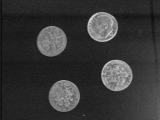
\includegraphics{images/outshrink.png}
				\label{fig:shrink}
			\end{figure}

		\end{description}


	\item{\textsc{reflectImage}}
		\begin{description}

\begin{lstlisting}
void reflectImage( bool, const ImageType& );
\end{lstlisting}

			\item{Purpose}

				reflects image by moving the pixel to N or M
				minus the current row or column
				depending on the value of the flag
				(true being a horizontal reflection and
				false being a vertical reflection)

			\item{Input}

				\begin{itemize}

					\item{flag}

						The flag that sets either vertical or
						horizontal reflection

					\item{ImageType old}

						The image to be reflected

				\end{itemize}

			\item{Output}

				None

			\item{Assumptions}

				Assumes nothing, but it makes sense to have an initialized
				image to reflect

			\item{Example}

				See figure~\ref{fig:reflect} on page~\pageref{fig:reflect}

				\begin{figure}[p]
					\centering
					\caption{reflectImage Example}
				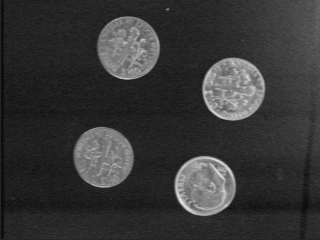
\includegraphics{images/outreflect.png}
				\label{fig:reflect}
			\end{figure}

		\end{description}


	\item{\textsc{translateImage}}
		\begin{description}

\begin{lstlisting}
void translateImage( int, const ImageType& );
\end{lstlisting}

			\item{Purpose}

				Translate the image down to the right,
				any part that goes out of the screen is
 				not calculated.  Checkered background from
				setImageInfo is retained.

			\item{Input}

				\begin{itemize}

					\item{t}

						The integer value of the translation. The
						translation will occur down and 
						to the right 't' pixels

					\item{ImageType old}

						The image to be translated

				\end{itemize}

			\item{Output}

				None

			\item{Assumptions}

				No assumptions are made, but it makes sense to have
				an initialized image

			\item{Example}

				See figure~\ref{fig:trans} on page~\pageref{fig:trans}

				\begin{figure}[p]
					\centering
					\caption{translateImage Example}
				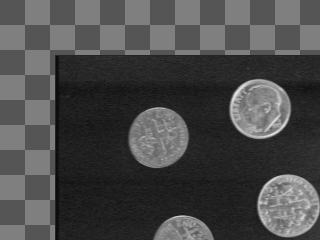
\includegraphics{images/outtrans.png}
				\label{fig:trans}
			\end{figure}

		\end{description}


	\item{\textsc{rotateImage}}
		\begin{description}

\begin{lstlisting}
void rotateImage( int, const ImageType& );
\end{lstlisting}

			\item{Purpose}

				Rotate the image clockwise using bi-linear
				interpolation, basically traversing
				the entire image going from the destination 
				to the source by using the
				in reverse (which is why its clockwise). 
				Once a location is determined the
				surrounding pixels are used to calculate 
				intermediate values between the
				pixels, this gives a pretty smooth rotate.

			\item{Input}

				\begin{itemize}

					\item{theta}

						The degrees to rotate. This is converted
						to radians inside the function

					\item{ImnageType old}

						The image to be rotated

				\end{itemize}

			\item{Output}

				None

			\item{Assumptions}

				Assumes that theta is in degrees because theta is
				converted to radians from degrees inside the function
				for the use of the trig functions.
				It is also assumed that the image has been initialized
				before the function call. It is also assumed that theta
				is between 0 and 360.

			\item{Example}

				See figure~\ref{fig:rotate} on page~\pageref{fig:rotate}

				\begin{figure}[p]
					\centering
					\caption{rotateImage Example}
				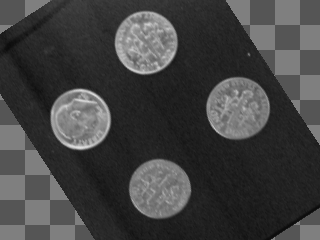
\includegraphics{images/outrotate.png}
				\label{fig:rotate}
			\end{figure}

		\end{description}


	\item{\textsc{operator+}}
		\begin{description}

\begin{lstlisting}
ImageType& operator+ ( const ImageType& );
\end{lstlisting}

			\item{Purpose}

				
				Sum two images together, basically just finding
				the average pixel value of
				every pixel between two images.  Throws an
				exception if dimensions of both
				images don't match

			\item{Input}

				\begin{itemize}
						
					\item{ImageType rhs}

						This is the image to be added to
						'this' image

				\end{itemize}

			\item{Output}

				ImageType object to chain additions

			\item{Assumptions}

				It is assumed that each image have the same dimensions.
				However, if the images do not have the same dimensions,
				then a string is thrown stating that the images do
				not have the same dimensions. It is not necessary to have
				each image initialized, but it makes senses
				that they would each be initialized.

			\item{Example}

				See figure~\ref{fig:operator+} on page~\pageref{fig:operator+}

				\begin{figure}[p]
					\centering
					\caption{operator+ Example}
				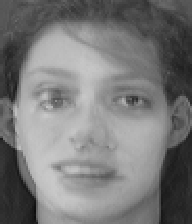
\includegraphics{images/outasum.png}
				\label{fig:operator+}
			\end{figure}


		\end{description}


	\item{\textsc{operator-}}
		\begin{description}

\begin{lstlisting}
ImageType& operator- ( const ImageType& );
\end{lstlisting}

			\item{Purpose}

				subtract two images from each other to see the 
				differences, if the magnitude of
				the difference is less then Q/6 then the pixel
				is replaced with black,	otherwise white is used. 
				This seems to help reduce 
				the amount of noise in the pictures

			\item{Input}

				\begin{itemize}

					\item{ImageType rhs}

						This is the image to be subtracted from
						'this' image

				\end{itemize}

			\item{Output}

				ImageType is returned to allow chaining of subtraction

			\item{Assumptions}

				It is assumed that each image have the same dimensions.
				However, if the images do not have the same dimensions,
				then a string is thrown stating that the images do
				not have the same dimensions. It is not necessary to have
				each image initialized, but it makes senses
				that they would each be initialized.

			\item{Example}

				See figure~\ref{fig:subtract} on page~\pageref{fig:subtract}
				
				\begin{figure}[p]
					\centering
					\caption{operator- Example}
				
\includegraphics[scale=.75]{images/outsubtract.png}
				\label{fig:subtract}
			\end{figure}

		\end{description}


	\item{\textsc{negateImage}}
		\begin{description}

\begin{lstlisting}
void negateImage();
\end{lstlisting}

			\item{Purpose}

				This function simply subtracts the current pixel
				value from the max value of
				the pixel, thus negating the image

			\item{Input}

				None

			\item{Output}

				None

			\item{Assumptions}

				Nothing is assumed

			\item{Example}

				See figure~\ref{fig:negative} on page~\pageref{fig:negative}

				\begin{figure}[h!]
					\centering
					\caption{negateImage Example}
				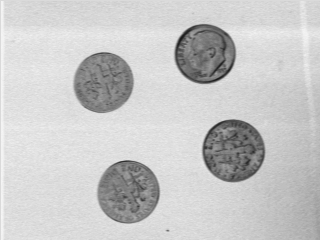
\includegraphics{images/outnegative.png}
				\label{fig:negative}
			\end{figure}

		\end{description}


\end{description}

\subsection{driver.cpp}

\begin{description}

	\item{\textsc{showmenu}}

		\begin{lstlisting}

	int showMenu( WINDOW *&, const char[], int, int, int, int, 
	    char[][NAME_LEN], int, bool=false );
		\end{lstlisting}

		\begin{description}
			\item{Purpose}
				
 				This is the function which builds the scrolling menu system, this simply
				creates a curses window and puts all the options stored in menuStr onto the
				window, it then waits for the user to press UP, DOWN, or RETURN before
				reacting.  The parameters allow menus to be different widths, heights, and
				locations.  A few constants can be changed to change the colors of the window.

			\item{Input}
				
				\begin{itemize}

					\item{*\&menu}

						An un-initialized window pointer.

					\item{title[]}

						A string to be the title.

					\item{height and width}

						The height and width of the menu.

					\item{locY and locX}
						
						The y and x locations of the menu's upper left corner.

					\item{menuStr[][NAME\_LEN] }

						A list of c-style strings to be used in the menu.
						
					\item{choices}
					
						The number of strings in menuStr.

					\item{erase}
						
						A bool value which says if the last choice is left highlighted.
						Default value is true.

				\end{itemize}

			\item{Output}
				
				Display a window with menu options, let user choose and
				return the index of that choice.

			\item{Assumptions}

				Assumes that window is un-initialized and will be destructed
				by calling function.

			\item{Example}

				See figure~\ref{fig:menu} on page~\pageref{fig:menu}

				\begin{figure}[p]
					\centering
					\caption{The Main Menu}
					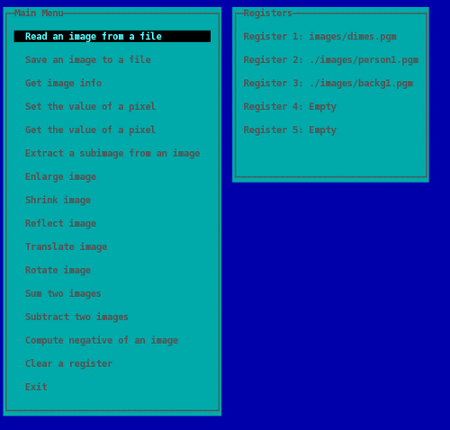
\includegraphics{images/menu.png}
					\label{fig:menu}
				\end{figure}

		\end{description}


	\item{\textsc{showregs}}

		\begin{lstlisting}

	void showRegs( WINDOW *&, const bool[], 
	const char[][NAME_LEN] );	
		\end{lstlisting}

		\begin{description}
			\item{Purpose}

 				Display a window of registers next to the main menu (or wherever the constants
				dictate).

			\item{Input}
			
				\begin{itemize}

					\item{*\&regWin}
						
						An un-initialized window pointer.

					\item{loaded[]}

						A list of bools representing which registers are loaded.

					\item{names[][NAMES\_LEN]}

						A list of the names of each register.

				\end{itemize}

			\item{Output}

				Displays a window next to main of all the registers.

			\item{Assumptions}

				This allocates memory for a WINDOW but it doesn't delete it.

		\end{description}


	\item{\textsc{drawwindow}}

		\begin{lstlisting}

	void drawWindow( WINDOW *&, const char[], 
		int, int, int, int, short=MENU_BACKGROUND, 
		short=MENU_FOREGROUND );
		\end{lstlisting}

		\begin{description}
			\item{Purpose}

				This function simply draws an empty window with a given title, height, width,
				x, and y locations.  The colors have default values but can be changed if
				oddly colored windows are wanted.

			\item{Input}

				\begin{itemize}

					\item{*\&win}

						An un-initialized window pointer.

					\item{title[]}

						A c-style string.

					\item{height and width}

						The height and width of the desired window.

					\item{y and x}

						The y and x locations of the upper left corner.

					\item{bgColor and fgColor}

						The background and foreground colors, both have default values equal
						to the menu colors defined as constants.

				\end{itemize}

			\item{Output}

				Displays a empty window with a border and title using the
				given parameters.

			\item{Assumptions}

				This allocates memory for a WINDOW but it doesn't delete it.

		\end{description}


	\item{\textsc{deletemenu}}

		\begin{lstlisting}

	void deleteMenu( WINDOW *& );
		\end{lstlisting}

		\begin{description}
			\item{Purpose}

				This basically clears the entire screen after deleting the window that is
				passed.

			\item{Input}

				\begin{itemize}

					\item{*\&menu}

						A window pointer which has been initialized.	

				\end{itemize}

			\item{Output}

				De-allocate memory for the window pointer and refresh the
				main screen.

			\item{Assumptions}

				Assumes WINDOW object is initialized before calling.


		\end{description}


	\item{\textsc{processentry}}

		\begin{lstlisting}

	void processEntry( ImageType[], bool[], 
	char[][NAME_LEN], int );
		\end{lstlisting}

		\begin{description}
			\item{Purpose}

				This is the function that decides where to go depending on the choice in the
				main menu.  The reason it has all the parameters is for passing to the
				subsequent functions that will be using them.

			\item{Input}

				\begin{itemize}

					\item{img[]}

						A list of images that are stored in the registers.

					\item{loaded[]}

						A list of bools that represent if each register is loaded.

					\item{name[][NAME\_LEN]}

						The names of all the registers as c strings.

					\item{choice}
				
						The choice the user made at the main menu.

				\end{itemize}

			\item{Output}

				Depending on the value of choice, call a function to do some image
				manipulation.

			\item{Assumptions}

				Assumes value $\geq$ 0 and $<$ MENU\_OPTIONS, not that anything
				will crash if its not true, but nothing will happen, also
				assumes that names contain valid c strings.

		\end{description}



	\item{\textsc{stdwindow}}

		\begin{lstlisting}

	void stdWindow( WINDOW *&, const char[] );
		\end{lstlisting}

		\begin{description}
			\item{Purpose}

				This just builds the window used for message box, this function is just to
				simplify the plethora of other functions that use this.
				
			\item{Input}
				
				\begin{itemize}

					\item{newWin}

						An un-initialized window pointer.

					\item{title[]}

						A c style string.

				\end{itemize}

			\item{Output}

				Displays a window in the standard text box location with
				the title and a border.

			\item{Assumptions}

				The window object is initialized here but not deleted, this
				is left up to the calling function.

		\end{description}



	\item{\textsc{promptforreg}}

		\begin{lstlisting}

	int promptForReg( bool[], char[][NAME_LEN], 
		const bool = true, int=1, int=MENU_WIDTH+3 );
		\end{lstlisting}

		\begin{description}
			\item{Purpose}
				
				This is the function that calls the menu for the register prompt, it can be
				called in different locations (like in addImg and subImg) but has a default
				defined by some global constants.  The function creates a list of registers
				and adds the "Back" option as the final option, this way the user has the
				option to cancel choosing a register.  Although in the program it looks like
				the register display and register choosing window are the same, this menu
				overlaps the other menu to make it seem like control is transferring to another
				window.

			\item{Input}

				\begin{itemize}

					\item{loaded[]}

						A list of flags indicating which registers are loaded.

					\item{name[][NAME\_LEN]}

						A list of names of each register.

					\item{check}

						A flag used to indicate weather registers that aren't loaded are valid.

					\item{y and x}

						The y and x locations of the menu, default values are defined for this.

				\end{itemize}

			\item{Output}
				
				Display a menu with the registers in it, allowing user to
				choose a register.

			\item{Assumptions}

				Assumes that names are already set to valid c strings.

		\end{description}



	\item{\textsc{promptforfilename}}

		\begin{lstlisting}

	int promptForFilename( const char[], 
		const char[], char[] );
		\end{lstlisting}

		\begin{description}
			\item{Purpose}

				Create a message box and prompt the user for a string value with given prompt.

			\item{Input}

				\begin{itemize}

					\item{title[]}

						The title of the prompt window as a c style string.

					\item{prompt[]}

						The prompting message.

					\item{str[]}

						A string in which to store output into.

				\end{itemize}

			\item{Output}

				Sets the final parameter equal to the file name the user
				chooses and returns the length.

			\item{Assumptions}

				Assumes first 2 parameters are valid c strings and that
				the final parameter is a string of at least length 16 plus
				the length of the file path declared as a constant.

		\end{description}



	\item{\textsc{promptforloc}}

		\begin{lstlisting}

	void promptForLoc( const char[], ImageType&, int&, int& );
		\end{lstlisting}

		\begin{description}
			\item{Purpose}

				This function prompts the user for a location (both row and column) and sets
				the valid points equal to row or col.  If -1 is returned in either location
				it means user choose to cancel the prompt.  The validity of the points is
				calculated by the image object it is passed.  The image properties are
				calculated and then used to determine the bounds of row and column.

			\item{Input}

				\begin{itemize}

					\item{title[]}

						The title of the prompt window as a c style string.

					\item{\&img}

						This is just so the dimensions of the image can be obtained.

					\item{\&row and \&col}

						Used to store the user's input values.

				\end{itemize}

			\item{Output}

				Sets two reference parameters equal to row and column of
				users choice.

			\item{Assumptions}

				Assumes image is initialized and has a valid height and width
				also that first parameter is a valid c string.

		\end{description}



	\item{\textsc{promptforpixvalue}}

		\begin{lstlisting}

	int promptForPixValue( const char[], const char[], int );
		\end{lstlisting}

		\begin{description}
			\item{Purpose}

				Prompt for a pixel value which is from 0 to maxVal, if not display message
				box and re-prompt user until valid choice is made.

			\item{Input}

				\begin{itemize}
					
					\item{title[]}

						The title of the prompt window as a c style string.

					\item{prompt[]}

						The prompting message.

					\item{maxVal}

						The maximum value allowed to input.

				\end{itemize}

			\item{Output}

				Prompts user in message window and returns the value when
				the user inputs a valid value(-1 indicates cancel).

			\item{Assumptions}

				Assumes that first 2 parameters are valid c strings.

		\end{description}



	\item{\textsc{promptforscalevalue}}

		\begin{lstlisting}

	int promptForScaleValue( const char[], const char[], int );
		\end{lstlisting}

		\begin{description}
			\item{Purpose}

				This function prompts the user for a scale value and checks to make sure it
				is not greater than maxVal and not less than 2.  This is used in the enlarge
				and shrink functions.

			\item{Input}

				\begin{itemize}
					
					\item{title[]}

						The title of the prompt window as a c style string.

					\item{prompt[]}

						The prompting message.

					\item{maxVal}

						The maximum value allowed to input.

				\end{itemize}

			\item{Output}

				Prompts user in message window and returns the value when
				the user inputs a valid value(-1 indicates cancel).

			\item{Assumptions}

				Assumes that first 2 parameters are valid c strings.

		\end{description}


	\item{\textsc{promptformirror}}

		\begin{lstlisting}

	char promptForMirror( const char[], const char[] );
		\end{lstlisting}

		\begin{description}
			\item{Purpose}

				Prompt the user for the characters h, v, or c (not case sensitive) and return
				the value as soon as one of the 3 is pressed.

			\item{Input}

				\begin{itemize}
					
					\item{title[]}

						The title of the prompt window as a c style string.

					\item{prompt[]}

						The prompting message.

				\end{itemize}

			\item{Output}

				Returns users choice as a char.

			\item{Assumptions}

				Both parameters are valid c strings.

		\end{description}


	\item{\textsc{promptforangle}}

		\begin{lstlisting}

	int promptForAngle( const char[], const char[] );
		\end{lstlisting}

		\begin{description}
			\item{Purpose}

				Prompt user for a valid angle using a message box, make sure input is between
				0 and 360, if not display a message box and then re-prompt.

			\item{Input}

				\begin{itemize}
					
					\item{title[]}

						The title of the prompt window as a c style string.

					\item{prompt[]}

						The prompting message.

				\end{itemize}

			\item{Output}

				Returns the user angle choice.

			\item{Assumptions}

				Both parameters are valid c strings.

		\end{description}


	\item{\textsc{messagebox}}

		\begin{lstlisting}

	void messageBox( const char[], const char[] );
		\end{lstlisting}

		\begin{description}
			\item{Purpose}

				Displays a message box in the center of the screen with
				the message displayed in it.

			\item{Input}

				\begin{itemize}
					
					\item{title[]}

						The title of the window as a c style string.

					\item{msg[]}

						The message to be displayed in the message box.

				\end{itemize}


			\item{Output}
				
				Displays a message box in the center of the screen with
				the message displayed in it, then waits for the user to press
				return before continuing.

			\item{Assumptions}

				Assumes both parameters are valid c strings.

		\end{description}



	\item{\textsc{fillregs}}

		\begin{lstlisting}

	void fillRegs( ImageType[], bool[], char[][NAME_LEN], 
		int, char** );
		\end{lstlisting}

		\begin{description}
			\item{Purpose}

				This displays a simple message box to the screen with the given title and msg
				inside of it, it waits for the user to press RETURN before returning to
				calling function.

			\item{Input}

				\begin{itemize}

					\item{img[]}

						A list of all the images stored in the registers.

					\item{loaded[]}

						A list of bools representing if each register is loaded.

					\item{name[][NAME\_LEN]}

						A list of names of every register.
					
					\item{argc}

						The number of strings in argv.

					\item{**argv}

						The parameters passed to main.

				\end{itemize}

			\item{Output}

				Sets valid arguments to registers (loading images) and
				clears the rest of the registers.

			\item{Assumptions}

				Assumes that char** is a valid list of strings with int
				rows.

		\end{description}



	\item{\textsc{clearregisters}}

		\begin{lstlisting}

	void clearRegister( ImageType[], bool[], 
		char[][NAME_LEN] );
		\end{lstlisting}

		\begin{description}
			\item{Purpose}

				Prompt for a register that is filled and then clear it.
				
			\item{Input}

				\begin{itemize}

					\item{img[]}

						A list of all the images stored in the registers.

					\item{loaded[]}

						A list of bools representing if each register is loaded.

					\item{name[][NAME\_LEN]}

						A list of names of every register.

				\end{itemize}

			\item{Output}

				Prompt the user for which register to use, then if necessary
				prompt for additional information and call the function
				in ImageType that will allow the image in that register to
				be manipulated.

			\item{Assumptions}

				Assumes all names in the c string list are valid c
				strings and the bools coincide with the image types that
				reference the same index.

		\end{description}



	\item{\textsc{loadimage}}

		\begin{lstlisting}

	void loadImage( ImageType[], bool[], char[][NAME_LEN] );
		\end{lstlisting}

		\begin{description}
			\item{Purpose}

				Prompt the user for a register to load to, then let them choose from a list
				of the .pgm files in the local images directory (defined as a constant).

			\item{Input}

				\begin{itemize}

					\item{img[]}

						A list of all the images stored in the registers.

					\item{loaded[]}

						A list of bools representing if each register is loaded.

					\item{name[][NAME\_LEN]}

						A list of names of every register.

				\end{itemize}

			\item{Output}

				Prompt the user for which register to use, then if necessary
				prompt for additional information and call the function
				in ImageType that will allow the image in that register to
				be manipulated.

			\item{Assumptions}

				Assumes all names in the c string list are valid c
				strings and the bools coincide with the image types that
				reference the same index.

		\end{description}



	\item{\textsc{saveimage}}

		\begin{lstlisting}

	void saveImage( ImageType[], bool[], char[][NAME_LEN] );
		\end{lstlisting}

		\begin{description}
			\item{Purpose}

				Save image from a register to the local images directory, prompting user for
				register and file name.

			\item{Input}

				\begin{itemize}

					\item{img[]}

						A list of all the images stored in the registers.

					\item{loaded[]}

						A list of bools representing if each register is loaded.

					\item{name[][NAME\_LEN]}

						A list of names of every register.

				\end{itemize}

			\item{Output}

				Prompt the user for which register to use, then if necessary
				prompt for additional information and call the function
				in ImageType that will allow the image in that register to
				be manipulated.

			\item{Assumptions}

				Assumes all names in the c string list are valid c
				strings and the bools coincide with the image types that
				reference the same index.

		\end{description}



	\item{\textsc{getimageinfo}}

		\begin{lstlisting}

	void getImageInfo( ImageType[], bool[], char[][NAME_LEN] );
		\end{lstlisting}

		\begin{description}
			\item{Purpose}

				Simply retrieve image information and display to a window below the registers
				The data being displayed is the Register number, Image Height, Width, Q value,
				and average gray value.

			\item{Input}

				\begin{itemize}

					\item{img[]}

						A list of all the images stored in the registers.

					\item{loaded[]}

						A list of bools representing if each register is loaded.

					\item{name[][NAME\_LEN]}

						A list of names of every register.

				\end{itemize}

			\item{Output}

				Prompt the user for which register to use, then if necessary
				prompt for additional information and call the function
				in ImageType that will allow the image in that register to
				be manipulated.

			\item{Assumptions}

				Assumes all names in the c string list are valid c
				strings and the bools coincide with the image types that
				reference the same index.

		\end{description}



	\item{\textsc{setpixel}}

		\begin{lstlisting}

	void setPixel( ImageType[], bool[], char[][NAME_LEN] );
		\end{lstlisting}

		\begin{description}
			\item{Purpose}

				Prompt user for a register then a pixel location (row, col) and then the pixel
				value to change that pixel to.

			\item{Input}

				\begin{itemize}

					\item{img[]}

						A list of all the images stored in the registers.

					\item{loaded[]}

						A list of bools representing if each register is loaded.

					\item{name[][NAME\_LEN]}

						A list of names of every register.

				\end{itemize}

			\item{Output}

				Prompt the user for which register to use, then if necessary
				prompt for additional information and call the function
				in ImageType that will allow the image in that register to
				be manipulated.

			\item{Assumptions}

				Assumes all names in the c string list are valid c
				strings and the bools coincide with the image types that
				reference the same index.

		\end{description}



	\item{\textsc{getpixel}}

		\begin{lstlisting}

	void getPixel( ImageType[], bool[], char[][NAME_LEN] );
		\end{lstlisting}

		\begin{description}
			\item{Purpose}

				Return the value of a pixel in a selected image to the user.

			\item{Input}

				\begin{itemize}

					\item{img[]}

						A list of all the images stored in the registers.

					\item{loaded[]}

						A list of bools representing if each register is loaded.

					\item{name[][NAME\_LEN]}

						A list of names of every register.

				\end{itemize}

			\item{Output}

				Prompt the user for which register to use, then if necessary
				prompt for additional information and call the function
				in ImageType that will allow the image in that register to
				be manipulated.

			\item{Assumptions}

				Assumes all names in the c string list are valid c
				strings and the bools coincide with the image types that
				reference the same index.

		\end{description}



	\item{\textsc{extractsub}}

		\begin{lstlisting}

	void extractSub( ImageType[], bool[], char[][NAME_LEN] );
		\end{lstlisting}

		\begin{description}
			\item{Purpose}

				After getting the image to manipulate, prompt for two corners to make a
				subimage out of, if the lower right corner is above or left of the upper
				right corner re-prompt for valid points

			\item{Input}

				\begin{itemize}

					\item{img[]}

						A list of all the images stored in the registers.

					\item{loaded[]}

						A list of bools representing if each register is loaded.

					\item{name[][NAME\_LEN]}

						A list of names of every register.

				\end{itemize}

			\item{Output}

				Prompt the user for which register to use, then if necessary
				prompt for additional information and call the function
				in ImageType that will allow the image in that register to
				be manipulated.

			\item{Assumptions}

				Assumes all names in the c string list are valid c
				strings and the bools coincide with the image types that
				reference the same index.

		\end{description}



	\item{\textsc{enlargeimg}}

		\begin{lstlisting}

	void enlargeImg( ImageType[], bool[], char[][NAME_LEN] );
		\end{lstlisting}

		\begin{description}
			\item{Purpose}

				This function prompts the user for a scale value to enlarge an image by, it
				makes sure the scale value does not make the image larger than MAX\_IMG value
				because it may cause a stack overflow.

			\item{Input}

				\begin{itemize}

					\item{img[]}

						A list of all the images stored in the registers.

					\item{loaded[]}

						A list of bools representing if each register is loaded.

					\item{name[][NAME\_LEN]}

						A list of names of every register.

				\end{itemize}

			\item{Output}

				Prompt the user for which register to use, then if necessary
				prompt for additional information and call the function
				in ImageType that will allow the image in that register to
				be manipulated.

			\item{Assumptions}

				Assumes all names in the c string list are valid c
				strings and the bools coincide with the image types that
				reference the same index.

		\end{description}



	\item{\textsc{shrinkimg}}

		\begin{lstlisting}

	void shrinkImg( ImageType[], bool[], char[][NAME_LEN] );
		\end{lstlisting}

		\begin{description}
			\item{Purpose}

				The same as enlarge except it shrinks the image making sure it never gets
				smaller than MIN\_IMG.  This is because some image viewers won't open images
				as small as 2x2 (xv for example).

			\item{Input}

				\begin{itemize}

					\item{img[]}

						A list of all the images stored in the registers.

					\item{loaded[]}

						A list of bools representing if each register is loaded.

					\item{name[][NAME\_LEN]}

						A list of names of every register.

				\end{itemize}

			\item{Output}

				Prompt the user for which register to use, then if necessary
				prompt for additional information and call the function
				in ImageType that will allow the image in that register to
				be manipulated.

			\item{Assumptions}

				Assumes all names in the c string list are valid c
				strings and the bools coincide with the image types that
				reference the same index.

		\end{description}



	\item{\textsc{reflectimg}}

		\begin{lstlisting}

	void reflectImg( ImageType[], bool[], char[][NAME_LEN] );
		\end{lstlisting}

		\begin{description}
			\item{Purpose}

				Prompt user for a direction to reflect an image then reflect the image and
				store it back in the original register image.

			\item{Input}

				\begin{itemize}

					\item{img[]}

						A list of all the images stored in the registers.

					\item{loaded[]}

						A list of bools representing if each register is loaded.

					\item{name[][NAME\_LEN]}

						A list of names of every register.

				\end{itemize}

			\item{Output}

				Prompt the user for which register to use, then if necessary
				prompt for additional information and call the function
				in ImageType that will allow the image in that register to
				be manipulated.

			\item{Assumptions}

				Assumes all names in the c string list are valid c
				strings and the bools coincide with the image types that
				reference the same index.

		\end{description}



	\item{\textsc{translateimg}}

		\begin{lstlisting}

	void translateImg( ImageType[], bool[], char[][NAME_LEN] );
		\end{lstlisting}

		\begin{description}
			\item{Purpose}
			
				This prompts the user for how far to translate the image, then calls the
				translate function which moves the image down to the right 't' number of
				pixels.  Also Won't let user choose t value that would move image totally off
				the screen.

			\item{Input}

				\begin{itemize}

					\item{img[]}

						A list of all the images stored in the registers.

					\item{loaded[]}

						A list of bools representing if each register is loaded.

					\item{name[][NAME\_LEN]}

						A list of names of every register.

				\end{itemize}

			\item{Output}

				Prompt the user for which register to use, then if necessary
				prompt for additional information and call the function
				in ImageType that will allow the image in that register to
				be manipulated.

			\item{Assumptions}

				Assumes all names in the c string list are valid c
				strings and the bools coincide with the image types that
				reference the same index.

		\end{description}



	\item{\textsc{rotateimg}}

		\begin{lstlisting}

	void rotateImg( ImageType[], bool[], char[][NAME_LEN] );
		\end{lstlisting}

		\begin{description}
			\item{Purpose}

				This prompts the user for an angle theta which will rotate the image counter 
				clockwise by theta degrees.  The input is only valid from 0 to 360 which
				should cover all possibilities.

			\item{Input}

				\begin{itemize}

					\item{img[]}

						A list of all the images stored in the registers.

					\item{loaded[]}

						A list of bools representing if each register is loaded.

					\item{name[][NAME\_LEN]}

						A list of names of every register.

				\end{itemize}

			\item{Output}

				Prompt the user for which register to use, then if necessary
				prompt for additional information and call the function
				in ImageType that will allow the image in that register to
				be manipulated.

			\item{Assumptions}

				Assumes all names in the c string list are valid c
				strings and the bools coincide with the image types that
				reference the same index.

		\end{description}



	\item{\textsc{sumimg}}

		\begin{lstlisting}

	void sumImg( ImageType[], bool[], char[][NAME_LEN] );
		\end{lstlisting}

		\begin{description}
			\item{Purpose}

				Prompt for 2 images and attempt to sum them, there is no size checking because
				operator+ will throw a string which will be handled by main if sizes of the
				two images are different.

			\item{Input}

				\begin{itemize}

					\item{img[]}

						A list of all the images stored in the registers.

					\item{loaded[]}

						A list of bools representing if each register is loaded.

					\item{name[][NAME\_LEN]}

						A list of names of every register.

				\end{itemize}

			\item{Output}

				Prompt the user for which register to use, then if necessary
				prompt for additional information and call the function
				in ImageType that will allow the image in that register to
				be manipulated.

			\item{Assumptions}

				Assumes all names in the c string list are valid c
				strings and the bools coincide with the image types that
				reference the same index.

		\end{description}



	\item{\textsc{subtractimg}}

		\begin{lstlisting}

	void subtractImg( ImageType[], bool[], char[][NAME_LEN] );
		\end{lstlisting}

		\begin{description}
			\item{Purpose}

				Prompt for 2 images and attempt to calculate the difference, there's no size
				checking here for the same reason sumImg doesn't do size checking

			\item{Input}

				\begin{itemize}

					\item{img[]}

						A list of all the images stored in the registers.

					\item{loaded[]}

						A list of bools representing if each register is loaded.

					\item{name[][NAME\_LEN]}

						A list of names of every register.

				\end{itemize}

			\item{Output}

				Prompt the user for which register to use, then if necessary
				prompt for additional information and call the function
				in ImageType that will allow the image in that register to
				be manipulated.

			\item{Assumptions}

				Assumes all names in the c string list are valid c
				strings and the bools coincide with the image types that
				reference the same index.

		\end{description}



	\item{\textsc{negate img}}

		\begin{lstlisting}

	void negateImg( ImageType[], bool[], char[][NAME_LEN] );
		\end{lstlisting}

		\begin{description}
			\item{Purpose}

				Prompt user for which image to negate and negate it, pretty simple function.

			\item{Input}

				\begin{itemize}

					\item{img[]}

						A list of all the images stored in the registers.

					\item{loaded[]}

						A list of bools representing if each register is loaded.

					\item{name[][NAME\_LEN]}

						A list of names of every register.

				\end{itemize}

			\item{Output}

				Prompt the user for which register to use, then if necessary
				prompt for additional information and call the function
				in ImageType that will allow the image in that register to
				be manipulated.

			\item{Assumptions}

				Assumes all names in the c string list are valid c
				strings and the bools coincide with the image types that
				reference the same index.

		\end{description}



	\item{\textsc{findlocalpgm}}

		\begin{lstlisting}

	int findLocalPGM( char **&filenames );
		\end{lstlisting}

		\begin{description}
			\item{Purpose}

				A somewhat brittle function that reads all the .pgm files from a local
				directory (defined as a constant) and places them into a dynamically
				allocated c style string array.

			\item{Input}

				\begin{itemize}

					\item{**filenames}
						
						A double char pointer that is uninitialized.

				\end{itemize}

			\item{Output}

				Allocates enough memory for a list of all the ".pgm" files
				in the local path specified by the FILELOC constant.  It
				then copies the file names to the array and returns the
				number of rows in the array.

			\item{Assumptions}

				Pointer parameter is not initialized, but will be in the function
				this means it needs to be de-allocated later.

		\end{description}


\end{description}

\subsection{cubicspline.h}

\begin{description}
	\item{\textsc{constructor}}

		\begin{lstlisting}

	cubicSpline();
		\end{lstlisting}

		\begin{description}
			\item{Purpose}

				Initialize everything to NULL and 0.

			\item{Input}

				None

			\item{Output}

				None

			\item{Assumptions}

				After this runs, all variables are zero.

		\end{description}


	\item{\textsc{constructor with parameters}}

		\begin{lstlisting}

	cubicSpline( int[], int );
		\end{lstlisting}

		\begin{description}
			\item{Purpose}

				Let object be initialized and create a linear and cubic spline based
				on the parameters.

			\item{Input}

				\begin{itemize}

					\item{points[]}

						The array of points to be interpolated.

					\item{num}

						The number of points in the array.

				\end{itemize}

			\item{Output}
			
				Sets the variables for both cubic and linear splines in the object.

			\item{Assumptions}

				It is assumed that there are at least 3 points, otherwise cubic splines can't
				be created with this algorithm.

		\end{description}


	\item{\textsc{destructor}}

		\begin{lstlisting}

	~cubicSpline();
		\end{lstlisting}

		\begin{description}
			\item{Purpose}

				Delete all dynamically allocated memory before object is removed.

			\item{Input}

				None

			\item{Output}

				None

			\item{Assumptions}

				None

		\end{description}


	\item{\textsc{create}}

		\begin{lstlisting}

	void create( int[], int );
		\end{lstlisting}

		\begin{description}
			\item{Purpose}

				Using the points make it possible to calculate a location along the
				piecewise function at a later time.  Creates a linear spline function.

			\item{Input}

				\begin{itemize}

					\item{points[]}

						A list of points to be used to interpolate.

					\item{num}

						The number of points.

				\end{itemize}

			\item{Output}

				Sets the object up so that linear approximations of intermediate values between
				the points can be obtained using the getVal() function.

			\item{Assumptions}

				There is at least 1 point.

		\end{description}


	\item{\textsc{createcubic}}

		\begin{lstlisting}

	void createCubic(int[], int);
		\end{lstlisting}

		\begin{description}
			\item{Purpose}

				Using the points make it possible to calculate a location along the
				piecewise function at a later time.  Creates a cubic spline function.

			\item{Input}
			
				\begin{itemize}

					\item{points[]}

						A list of points to be used to interpolate.

					\item{num}

						The number of points.

				\end{itemize}

			\item{Output}

				Sets the object up so that cubic approximations of intermediate values between
				the points can be obtained using the getCubicVal() function.

			\item{Assumptions}

				It is assumed that 3 or more points exist.

		\end{description}


	\item{\textsc{getval}}

		\begin{lstlisting}

	double getVal( double );
		\end{lstlisting}

		\begin{description}
			\item{Purpose}

				Returns an estimated value along the function, the spline function assumes
				that the first point lies at 0.0 and the final point lies at 100.0 with each
				point equally spaced.  Uses a linear spline.

			\item{Input}

				\begin{itemize}

					\item{x}

						A floating point value of the desired location along the function.

				\end{itemize}

			\item{Output}

				Returns the value of the intermediate approximation between the points.

			\item{Assumptions}

				Assumes a linear spline has been defined. a.k.a. the function create()
				has been called, initializing the spline.

		\end{description}


	\item{\textsc{getcubicval}}

		\begin{lstlisting}

	double getCubicVal( double );
		\end{lstlisting}

		\begin{description}
			\item{Purpose}

				Returns an estimated value along the function, the spline function assumes
				that the first point lies at 0.0 and the final point lies at 100.0 with each
				point equally spaced.  Uses a cubic spline.

			\item{Input}

				\begin{itemize}

					\item{x}

						A floating point value of the desired location along the function.

				\end{itemize}

			\item{Output}

				Returns the value of the intermediate approximation between the points.

			\item{Assumptions}

				Assumes a cubic spline has been defined. a.k.a. the function createCubic() has
				been called, initializing the spline.

		\end{description}


\end{description}

\subsection{imageIO.h}

\begin{description}
	\item{\textsc{readimageheader}}

		\begin{lstlisting}

	void readImageHeader( const char[], int&, 
		int&, int&, bool& );
		\end{lstlisting}

		\begin{description}
			\item{Purpose}

				Reads the image header and puts them into values that
				are passed by reference

			\item{Input}

				\begin{itemize}

					\item{fname[]}

						This is the name of the file stored
						as a C-style string

					\item{N}

						This is the number of rows in the image

					\item{M}

						This is the number of columns in
						the image

					\item{Q}

						This is the depth of the image

					\item{type}

						This makes sure that the file type is
						.pgm and not some other format
						
				\end{itemize}
						
						
			\item{Output}

				None

			\item{Assumptions}

				Assumes that a file exists and is in pgm format

		\end{description}


	\item{\textsc{readimage}}

		\begin{lstlisting}

	void readImage( const char[], ImageType& );
		\end{lstlisting}

		\begin{description}
			\item{Purpose}

				Reads the image into the image object from a file

			\item{Input}

				\begin{itemize}

					\item{fname[]}

						The C-style string to hold the image 
						file name

					\item{ImageType image}

						The image object that holds the
						image data

				\end{itemize}

			\item{Output}

				None

			\item{Assumptions}

				Assumes there is a file to be read and that the
				user has read access

		\end{description}


	\item{\textsc{writeimage}}

		\begin{lstlisting}

	void writeImage( const char[], ImageType& );
		\end{lstlisting}

		\begin{description}
			\item{Purpose}

				Writes the image to disk

			\item{Input}

				\begin{itemize}

					\item{fname[]}

						The C-style string to hold the image 
						file name

					\item{ImageType image}

						The image object that holds the
						image data

				\end{itemize}



			\item{Output}

				None

			\item{Assumptions}

				Assumes the user has write access to the
				destination folder

		\end{description}


\end{description}

\subsection{comp\_curses.h}
\begin{description}

	\item{\textsc{startcurses}}

		\begin{lstlisting}

	void startCurses();
		\end{lstlisting}

		\begin{description}
			\item{Purpose}

				This initializes the curses screen and its functions

			\item{Input}

				None

			\item{Output}

				None

			\item{Assumptions}

				No assumptions are made besides have a terminal
				capable of displaying curses correctly.

		\end{description}


	\item{\textsc{endcurses}}

		\begin{lstlisting}

	void endCurses();
		\end{lstlisting}

		\begin{description}
			\item{Purpose}

				This ends the curses screen and its functions

			\item{Input}

				None

			\item{Output}

				None

			\item{Assumptions}

				This assumes that curses has been initialized
				with startCurses()


		\end{description}


	\item{\textsc{setcolor}}

		\begin{lstlisting}

	void setColor( WINDOW*, int, int );
		\end{lstlisting}

		\begin{description}
			\item{Purpose}

				This sets the colors for stdscr

			\item{Input}

				\begin{itemize}

					\item{*somewin}

						This is the window pointer to set
						the colors to a specific window

					\item{cf}

						This is the first color (foreground)
						for the color pair to set in the window

					\item{cb}

						This is the second color (background)
						for the color pair to set in the window
						
				\end{itemize}	

			\item{Output}

				None

			\item{Assumptions}

				Assumes that screen has been initialized

		\end{description}


	\item{\textsc{screenwidth}}

		\begin{lstlisting}

	int screenWidth();
		\end{lstlisting}

		\begin{description}
			\item{Purpose}

				Returns the max screen x value 

			\item{Input}

				None

			\item{Output}

				The int value of the max x value for the entire terminal

			\item{Assumptions}

				Assumes startCurses() has been run

		\end{description}


	\item{\textsc{screenheigth}}

		\begin{lstlisting}

	int screenHeight();
		\end{lstlisting}

		\begin{description}
			\item{Purpose}

				Returns the max screen y value

			\item{Input}

				None

			\item{Output}

				The int value of the max y value for the entire terminal

			\item{Assumptions}

				Assumes startCurses() has been run

		\end{description}


	\item{\textsc{promptforint}}

		\begin{lstlisting}

	int promptForInt( WINDOW*, int, int, const char [] );
		\end{lstlisting}

		\begin{description}
			\item{Purpose}

				Prompts for an int at some int at some (x,y) coordinate

			\item{Input}

				\begin{itemize}

					\item{*somewin}

						Some window to prompt for the int in

					\item{y}

						The y coordinate at which to prompt
						for the int

					\item{x} 

						The x coordinate at which to prompt
						for the int

					\item{promptString[]}

						The string to display when prompting for
						the int
						
				\end{itemize}

			\item{Output}

				The integer value of the user's input

			\item{Assumptions}

				It is assumed that startCurses() has been run.
				The function has built in error checking to prevent
				bad data from being input

		\end{description}


	\item{\textsc{promptfordouble}}

		\begin{lstlisting}

	double promptForDouble( WINDOW*, int, int, const char[] );
		\end{lstlisting}

		\begin{description}
			\item{Purpose}

				Prompts for a double at some int at some (x,y) coordinate

			\item{Input}

				\begin{itemize}

					\item{*somewin}

						Some window to prompt for the double in

					\item{y}

						The y coordinate at which to prompt
						for the double

					\item{x} 

						The x coordinate at which to prompt
						for the double

					\item{promptString[]}

						The string to display when prompting for
						the double
						
				\end{itemize}



			\item{Output}

				The double value of the user's input

			\item{Assumptions}

				It is assumed that startCurses() has been run.
				The function has built in error checking to prevent
				bad data from being input (such as multiple periods)

		\end{description}


	\item{\textsc{promptforstring}}

		\begin{lstlisting}

	void promptForString( WINDOW *, int, int, 
		const char[], char[], int );
		\end{lstlisting}

		\begin{description}
			\item{Purpose}

				Prompts for a string at some (x,y) coordinate

			\item{Input}

				\begin{itemize}

					\item{*somewin}

						The window at which to prompt
						for the string

					\item{y}

						The y coordinate at which to prompt

					\item{x}

						The x coordinate at which to prompt

					\item{promptstring}

						The string to display when prompting
						for the string

					\item{str[]}

						The array for the string that is typed
						in by the user

					\item{len}

						The length of the string stored

				\end{itemize}

			\item{Output}

				None

			\item{Assumptions}

				It is assumed that startCurses() has been run.
				The function also accounts for backspaces and
				makes sure that only valid input is entered.

		\end{description}


\end{description}

\section{Bugs and Errors}

	During the creation of this program we ran into a multitude of bugs and errors.  Some of the biggest obstacles came
while implementing the main driver program.  Learning how curses works and finding way to make it do what was needed was
quite a challenge but also very rewarding.  One odd bug was that when the function wattron() was used to set to
highlight for the menu options it worked fine on one computer, but when it was used on Josiah's computer the
highlighting didn't show up.  The fix for this involved manually inverting the colors rather than just changing the
attribute.  This is a good example of how a program may act differently on different computers.

Another bug that we ran into was having trouble when enlarging images too much.  The way this was dealt with was to add a
global constant to the main driver which limited the size allowed to scale an image.  Although there weren't many actual
bugs while writing the image class, there was a huge amount of testing done to try and make the program as robust as
possible given the time limitation.

\section{What was Learned}

The most important thing learned in this assignment was the use of dynamic 2D arrays. This was not taught in the previous
semester of CS, so the concept of it was new to the students. This challenge did not sway them though. the students
quickly grasped the concepts of a dynamic 2D array and easily implemented it into the image class. The students were
then able to design the functions that manipulated the 2D array that in turn manipulated the image. This was an
important concept to grasp because without understanding the concepts of a 2D array, the students would not be able to
correctly develop algorithms that correctly manipulated the image. 

Another concept that the students learned was the knowledge of how images are stored. The students had first hand
experience with an image format and this knowledge allowed the students to have a greater understanding of how computers
and the data structures associated with file formats intertwine with the software developer. The students have more of
an appreciation for the necessity of data structures and the implications of designing easy to use and compact data
structures for the end user. 

One of the other concepts that the students learned was the ability to use ncurses in their program. This knowledge
allowed the students to create a very easy-to-use menu that is capable of multiple floating and scrollable menus. While
this part of the program was not needed, the students had a desire to learn more about C++ than what is being taught in
the class and brought it upon themselves to learn about ncurses. This knowledge has greatly improved their knowledge of
pointers and correct program structure because ncurses utilizes many pointers. The implementation of ncurses also becomes
very complex if there is not a clean program structure implemented. There are many facets of ncurses that are
intertwined, so the students made a clean and modular ncurses driver that is able to be easily read.

Since this was a group project, we felt that it would be fairly difficult to merge and maintain our code, so we decided
to learn and use git. Git is a revision control program that focuses on software development. It was developed by Linus
Torvalds for the development of the Linux kernel. Git has proved to be extremely useful in the management of the source
code. It did have a small learning curve, but once that was crossed, it has become one of the most valuable tools that I
know of.

\section{Division of Labor}

For the requirements that were asked for, each student did an equal amount of work. The students met very early and
divided up the required functions equally. Each student then implemented each function of the image class. Since the
students are at different levels of programming experience, one of the students went above the required implementation
to challenge himself. Josh implemented some advanced methods of manipulating the image using knowledge from a numerical
methods class that he has taken in the past. Josh also wrote the driver with the help of Josiah for feedback on how to
design the menu system. Both students studied and learned how the curses environment works and equally experimented with
the functionality of curses and its implementation into a menu system. For the documentation, Josiah wanted to go above
the normal implementation of a standard documentation and implemented a \LaTeX document that made the writing of the
documentation very easy and structured. Overall, the students contributed equally for their level of programming skill.

\section{Extra Credit}

	\subsection{Question 1}	

		\begin{description}

			\item{QUESTION:}

				The algorithm that you have to implement in this assignment to shrink an image
				is actually very simple and might not always produce good results. Can you think of a more
				effective solution?
			
			\item{ANSWER:}

				We used a method where instead of just taking samples we actually averaged all the pixel in each
				block that is truncated, that way no pixel is unaccounted for.  For example if the scale value was
				5, then blocks of 5x5 would be shrunk to 1x1.  The original method made it so that only the upper
				left corner of the 5x5 block would be sampled. 

				
		\end{description}

	\subsection{Question 2}	

		\begin{description}

			\item{QUESTION:}

				We have already discussed in class two practical difficulties associated with rotation: (a) the
				case where the transformed pixel coordinates fall outside the image and (b) the case
				where the transformed pixel coordinates are not integers. In the first case, we suggested simply
				ignoring the transformed pixel coordinates which fall outside the range. This is probably enough
				in most cases. In the second case, we suggested finding the nearest integer neighbors to r′ and c′.
				This approach, however, will not produce a value for every pixel in the output image. In other
				words, it will produce numerous "holes" in the rotated image where no value was computed. Can
				you suggest a way for dealing with this problem?

			\item{ANSWER:}

				To make up for holes in our images, did the opposite of what was originally suggested.  Instead of
				going from the source to the new location we took the new locations and went back to the original
				to see where that point should fall.  This is actually much easier than it sounds as only the
				index values of the pixel's needed to be reversed.  The one issue with this method is that instead
				of a counter-clockwise rotation, a clockwise rotation happens.  We fixed this problem by reversing
				the angle before making the calculation.  Another feature we added to rotate was that it estimates
				intermediate values so if the destination is looking for a value at (23.234, 43.23) a simple
				bi-linear algorithm is implemented to obtain the estimated value for that point based on the four
				points it falls around.

		\end{description}

	\subsection{Question 3}	

		\begin{description}

			\item{QUESTION:}
			
				This question is regarding image subtraction. By examining the difference image,
				you will notice some rather small non-zero values in image areas where there is not really any
				change (e.g., subtract "backg1.pgm" from "backg2.pgm" and look at the values of the difference
				image). These differences are due to sensor noise, slight changes in illumination and various
				other factors. Can you suggest of a way to deal with this problem?

			\item{ANSWER:}

				For image subtraction there were a few idea's that we had to reduce the amount of noise, but the
				one we ended up going with was to simply add a difference threshold.  This basically means that
				we made all pixels that differed by at least 43 (which is $\approx$ 255 $\div$ 6).  This does
				show some improvements for noticing differences in images without a lot of noise, although some
				noise is still there.
				
				See figures~\ref{fig:subnoisy} and~\ref{fig:subclear} on pages~\pageref{fig:subnoisy}
				and~\pageref{fig:subclear}
				
				An idea that we had, but didn't have time to implement was to look at each pixel after the threshold
				is made and remove any white pixel that doesn't have 3 neighbors, then run this over the image until
				no changes are made.  I don't know how this would react but we thought it was an interesting idea.

		\end{description}
	
	\subsection{Extras}

		\begin{description}

			\item{Final Thoughts}

				This section isn't required but we thought that it was important to explain all the extra features that
				were added to this project.  The biggest addition to the project was the addition of bi-cubic interpolation
				for enlargeImage().  This was done by Josh as more of a coding challenge, but worked out pretty well.  The
				type of spline used is a natural spline calculated using a Lagrange polynomial.  This method was chosen
				because it only has n-1 unknowns, rather than a normal polynomial interpolation which has 4 times as many
				unknowns.  It also allows a tridiagonal matrix to solve for all the unknowns, which is much faster than
				a normal matrix solving algorithm.

				Another addition to the project was the curses driver program.  This was done to make using the program a
				little more enjoyable and also to show some of the things that can be done with curses.  All in all these
				extra additions were an enjoyable challenge and I hope you enjoy them.

				See figure~\ref{fig:enlargecubic} and~\ref{fig:enlargestd} on page~\pageref{fig:enlargecubic}
				and~\pageref{fig:enlargestd}
				
				\begin{figure}[p]
					\centering
					\caption{enlarge without cubic Example}
					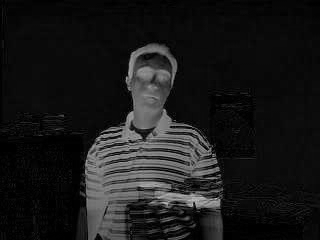
\includegraphics{images/subnoisy.png}
					\label{fig:subnoisy}
				\end{figure}
				
				\begin{figure}[p]
					\centering
					\caption{enlarge without cubic Example}
					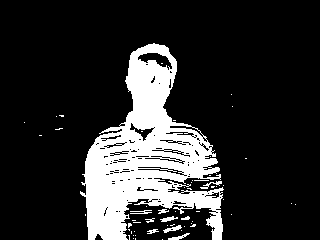
\includegraphics{images/subclear.png}
					\label{fig:subclear}
				\end{figure}

		\end{description}

\end{document}
